%=============================================================================
%  Post Image Processing in Ultrasound Simulation
%  Darshil Maniya  |  262SP009
%  Dept. of Electronics and Communication Engineering, NITK Surathkal
%=============================================================================
\documentclass[12pt,a4paper,oneside]{report}

%------------------------------ page geometry -------------------------------
\usepackage[left=1.2in,right=0.95in,top=0.95in,bottom=0.95in]{geometry}

%------------------------------ fonts & spacing -----------------------------
\usepackage{mathptmx}                 % Times New Roman text + math
\usepackage[T1]{fontenc}
\usepackage[utf8]{inputenc}
\usepackage{setspace}
\setstretch{1.08}
\setlength{\parindent}{0pt}
\setlength{\parskip}{3pt}

%------------------------------ packages ------------------------------------
\usepackage{amsmath,amssymb}
\AtBeginDocument{%
  \setlength{\abovedisplayskip}{6pt}\setlength{\belowdisplayskip}{6pt}%
  \setlength{\abovedisplayshortskip}{4pt}\setlength{\belowdisplayshortskip}{4pt}}
\usepackage{graphicx}
\usepackage{booktabs}
\usepackage{array}
\usepackage{multirow}
\usepackage[font=small,labelfont=bf,justification=centering]{caption}
\usepackage{subcaption}
\usepackage{float}
\renewcommand{\topfraction}{0.92}
\renewcommand{\bottomfraction}{0.85}
\renewcommand{\textfraction}{0.08}
\renewcommand{\floatpagefraction}{0.80}
\setlength{\textfloatsep}{10pt}
\setlength{\intextsep}{10pt}
\setlength{\abovecaptionskip}{5pt}
\usepackage[table]{xcolor}
\usepackage{tikz}
\usetikzlibrary{shapes.geometric,arrows.meta,positioning,calc,fit,backgrounds}
\usepackage{pgfplots}
\pgfplotsset{compat=1.17}
\usepackage{fancyhdr}
\usepackage{titlesec}
\usepackage{tocloft}
\usepackage{enumitem}
\usepackage{listings}
\usepackage[hidelinks,breaklinks=true]{hyperref}

%------------------------------ colours -------------------------------------
\definecolor{nitkblue}{HTML}{2479C6}
\definecolor{nitkorange}{HTML}{C55A11}
\definecolor{tabhead}{HTML}{DEEAF6}
\definecolor{tabalt}{HTML}{F2F2F2}
\definecolor{codebg}{HTML}{F7F7F7}

%------------------------------ headings ------------------------------------
\titleformat{\chapter}[display]
  {\normalfont\Large\bfseries\color{nitkblue}}
  {\Large CHAPTER \thechapter}{6pt}{\LARGE}
\titlespacing*{\chapter}{0pt}{-34pt}{12pt}
\titleformat{\section}{\normalfont\large\bfseries\color{nitkblue}}{\thesection}{1em}{}
\titleformat{\subsection}{\normalfont\normalsize\bfseries\color{nitkorange}}{\thesubsection}{1em}{}

%------------------------------ tighter TOC spacing --------------------------
\setlength{\cftbeforechapskip}{3pt}
\renewcommand{\cftchapafterpnum}{\vskip -1pt}
\renewcommand{\cftsecafterpnum}{\vskip -1pt}
\setlength{\cftparskip}{-1pt}

%------------------------------ headers/footers ------------------------------
\pagestyle{fancy}
\fancyhf{}
\renewcommand{\headrulewidth}{0.4pt}
\fancyhead[L]{\small\itshape Post Image Processing in Ultrasound Simulation}
\fancyhead[R]{\small\thepage}
\fancypagestyle{plain}{\fancyhf{}\renewcommand{\headrulewidth}{0pt}
  \fancyfoot[C]{\small\thepage}}

%------------------------------ listings ------------------------------------
\lstset{
  basicstyle=\ttfamily\scriptsize,
  backgroundcolor=\color{codebg},
  keywordstyle=\color{nitkblue}\bfseries,
  commentstyle=\color{gray}\itshape,
  stringstyle=\color{nitkorange},
  numbers=left, numberstyle=\tiny\color{gray}, numbersep=8pt,
  frame=single, rulecolor=\color{gray!40},
  breaklines=true, showstringspaces=false,
  language=Python, captionpos=b, xleftmargin=14pt
}

%------------------------------ tikz styles ---------------------------------
\tikzset{
  blk/.style   ={rectangle, rounded corners=3pt, draw=nitkblue, very thick,
                 fill=nitkblue!8, minimum width=2.9cm, minimum height=1.0cm,
                 align=center, font=\small},
  hblk/.style  ={rectangle, rounded corners=3pt, draw=nitkorange, very thick,
                 fill=nitkorange!12, minimum width=2.9cm, minimum height=1.0cm,
                 align=center, font=\small\bfseries},
  gblk/.style  ={rectangle, rounded corners=3pt, draw=green!45!black, very thick,
                 fill=green!12, minimum width=2.9cm, minimum height=1.0cm,
                 align=center, font=\small},
  dec/.style   ={diamond, aspect=1.9, draw=nitkorange, very thick,
                 fill=nitkorange!10, align=center, font=\scriptsize},
  io/.style    ={trapezium, trapezium left angle=70, trapezium right angle=110,
                 draw=gray!70!black, very thick, fill=gray!10,
                 align=center, font=\small, minimum height=0.85cm},
  ar/.style    ={-{Stealth[length=3mm]}, very thick, draw=gray!60!black}
}

%------------------------------ table helper --------------------------------
\newcolumntype{L}[1]{>{\raggedright\arraybackslash}p{#1}}
\newcolumntype{C}[1]{>{\centering\arraybackslash}p{#1}}

\begin{document}

%=============================================================================
%  TITLE PAGE
%=============================================================================
\begin{titlepage}
\centering
\vspace*{0.3cm}

{\Large\bfseries POST IMAGE PROCESSING IN\\[4pt] ULTRASOUND SIMULATION\par}

\vspace{0.5cm}
{\normalsize\itshape Module of the NITK-UsoundSim Project\par}

\vspace{0.35cm}
{\normalsize\itshape Seminar Report --- Course Code: EC787\par}

\vspace{0.9cm}
{\normalsize A Project Report submitted in partial fulfilment of the\\
requirements for the degree of\par}

\vspace{0.4cm}
{\large\bfseries MASTER OF TECHNOLOGY\par}

\vspace{0.3cm}
{\normalsize in\par}
\vspace{0.2cm}
{\large\bfseries SIGNAL PROCESSING AND MACHINE LEARNING\par}

\vspace{0.9cm}
{\normalsize\itshape submitted by\par}
\vspace{0.35cm}
{\large\bfseries DARSHIL MANIYA\par}
\vspace{0.15cm}
{\large (262SP009)\par}

\vspace{0.9cm}

\includegraphics[width=3.1cm]{figures/nitk_logo.png}

\vspace{0.7cm}
{\normalsize\bfseries DEPARTMENT OF ELECTRONICS AND\\[2pt]
COMMUNICATION ENGINEERING\par}
\vspace{0.3cm}
{\normalsize\bfseries NATIONAL INSTITUTE OF TECHNOLOGY KARNATAKA,\\[2pt]
SURATHKAL, MANGALORE -- 575025\par}

\vspace{0.6cm}
{\normalsize\bfseries 2026\par}
\end{titlepage}

%=============================================================================
%  FRONT MATTER
%=============================================================================
\pagenumbering{roman}
\setcounter{page}{2}

%---------------------------- declaration -----------------------------------
\chapter*{DECLARATION}
\addcontentsline{toc}{chapter}{Declaration}
\thispagestyle{plain}

I hereby declare that the report of the project work titled \textbf{``Post Image
Processing in Ultrasound Simulation''}, which is being submitted to the National
Institute of Technology Karnataka, Surathkal, in partial fulfilment of the
requirements for the award of the Degree of \textbf{Master of Technology} in the
Department of Electronics and Communication Engineering, is a bonafide report of
the work carried out by me. The material contained in this report has not been
submitted to any University or Institution for the award of any degree.

\vspace{0.8cm}
\begin{flushleft}
\textbf{Darshil Maniya}\\
Register Number: 262SP009\\[0.5cm]
Place: NITK, Surathkal \hspace{1.5cm} Date: \rule{3cm}{0.4pt}
\end{flushleft}

%---------------------------- certificate -----------------------------------
\vspace{1.0cm}
\section*{\centering CERTIFICATE}
\addcontentsline{toc}{chapter}{Certificate}

This is to certify that the project report titled \textbf{``Post Image Processing
in Ultrasound Simulation''} submitted by \textbf{Darshil Maniya} (Register Number:
262SP009) as the record of the work carried out by him, is accepted as the
\emph{Project Work Report} submission in partial fulfilment of the requirements
for the award of the degree of \textbf{Master of Technology} in the Department of
Electronics and Communication Engineering, National Institute of Technology
Karnataka, Surathkal.

\vspace{1.6cm}
\noindent
\begin{minipage}[t]{0.48\textwidth}
\rule{5cm}{0.4pt}\\
\textbf{Project Guide}\\
Dept. of E\&C Engineering\\
NITK Surathkal
\end{minipage}\hfill
\begin{minipage}[t]{0.48\textwidth}
\rule{5cm}{0.4pt}\\
\textbf{Chairman -- DPGC}\\
Dept. of E\&C Engineering\\
NITK Surathkal
\end{minipage}

%---------------------------- abstract --------------------------------------
\chapter*{ABSTRACT}
\addcontentsline{toc}{chapter}{Abstract}
\thispagestyle{plain}

Ultrasound is among the most widely used diagnostic imaging modalities because it
is inexpensive, portable, real-time and free of ionising radiation. Its principal
image-quality limitation is \emph{speckle} --- a granular interference pattern
produced when echoes from sub-resolution scatterers add coherently at the
transducer. Speckle is deterministic rather than random electronic noise, it is
present in every scan, and it obscures low-contrast lesions, blurs organ
boundaries and degrades the performance of automated analysis methods.

This report describes the \textbf{Post Image Processing} module of
\textbf{NITK-UsoundSim}, a software ultrasound imaging system developed by a
sixteen-member student team across eight modules. This module is the terminal
stage: it accepts the log-compressed, scan-converted B-mode image from the B-Mode
Image Formation module and returns a display-ready image in which speckle has
been suppressed without destroying diagnostically relevant structure. A
four-stage chain is proposed and implemented --- depth-gain normalisation,
despeckle filtering, contrast and edge restoration, and automated quality
assessment. Five classical filters (median, Lee, Speckle Reducing Anisotropic
Diffusion, Non-Local Means and wavelet soft thresholding) are implemented in
Python and compared quantitatively; no machine-learning model is used at any
stage.

Because the upstream dependency was unavailable during development, a synthetic
B-mode testbench was constructed for validation. It generates a sector-format
phantom containing an anechoic cyst, a hyperechoic lesion, a hypoechoic nodule
and point targets with fully developed Rayleigh speckle, and supplies a noise-free
ground-truth image permitting reference-based metrics.

On this testbench, SRAD achieved the best overall balance, raising the
contrast-to-noise ratio from 1.78 to 2.98 and the speckle signal-to-noise ratio
from 4.28 to 9.29 while retaining an edge-preservation index of 0.96. Non-Local
Means attained marginally higher noise suppression (SNR 9.77) but retained only
0.81 of the edge information and was the slowest method evaluated. SRAD is
therefore recommended as the default filter for the module.

\vspace{0.5cm}
\textbf{Keywords:} Ultrasound imaging, B-mode, speckle, despeckling, anisotropic
diffusion, SRAD, non-local means, contrast-to-noise ratio, image enhancement.

%---------------------------- acknowledgement -------------------------------
\chapter*{ACKNOWLEDGEMENT}
\addcontentsline{toc}{chapter}{Acknowledgement}
\thispagestyle{plain}

I express my sincere gratitude to my project guide in the Department of
Electronics and Communication Engineering, NITK Surathkal, for the continuous
guidance, technical direction and encouragement provided throughout this work, and
to the faculty of the Department for the academic environment and computational
resources that made this project possible.

I also thank my teammates on the NITK-UsoundSim project, particularly the Receiver
Beamforming and B-Mode Image Formation module teams, whose discussions shaped the
input specification adopted here. Finally, I thank my family and friends for their
constant support.

\vspace{1.2cm}
\begin{flushright}
\textbf{Darshil Maniya}\\
262SP009
\end{flushright}

%---------------------------- contents --------------------------------------
\clearpage
\begingroup
\small
\setcounter{tocdepth}{1}
\tableofcontents
\addcontentsline{toc}{chapter}{Table of Contents}
\endgroup

\clearpage
\listoffigures
\addcontentsline{toc}{chapter}{List of Figures}

\clearpage
\begingroup
\let\clearpage\relax
\listoftables
\addcontentsline{toc}{chapter}{List of Tables}
\vspace{10pt}

\section*{LIST OF ABBREVIATIONS}
\addcontentsline{toc}{chapter}{List of Abbreviations}
\endgroup

\begin{center}\small
\begin{tabular}{L{2.8cm} L{8.6cm}}
\toprule
\textbf{Abbreviation} & \textbf{Expansion}\\
\midrule
B-mode  & Brightness Mode\\
CLAHE   & Contrast Limited Adaptive Histogram Equalisation\\
CNR     & Contrast-to-Noise Ratio\\
DGC     & Depth Gain Compensation\\
EPI     & Edge Preservation Index\\
FWHM    & Full Width at Half Maximum\\
NLM     & Non-Local Means\\
PSF     & Point Spread Function\\
PSNR    & Peak Signal-to-Noise Ratio\\
RF      & Radio Frequency\\
ROI     & Region of Interest\\
SNR     & Signal-to-Noise Ratio\\
SRAD    & Speckle Reducing Anisotropic Diffusion\\
SSIM    & Structural Similarity Index Measure\\
TGC     & Time Gain Compensation\\
VCT     & Virtual Clinical Trial\\
\bottomrule
\end{tabular}
\end{center}

\clearpage
\pagenumbering{arabic}
\setcounter{page}{1}

%=============================================================================
\chapter{INTRODUCTION AND BACKGROUND}
\label{ch:intro}
%=============================================================================

\section{Background}

Medical ultrasound imaging uses high-frequency acoustic pulses, typically
2--15\,MHz, to visualise internal anatomy. A transducer array on the skin transmits
a focused pulse; a fraction of its energy is reflected at every interface where
acoustic impedance changes. The returning echoes are beamformed,
envelope-detected, log-compressed and mapped to grey levels to form the
brightness-mode (B-mode) image \cite{kang2015musiic}.

Ultrasound uses no ionising radiation, costs a small fraction of a computed
tomography or magnetic resonance system, is portable enough for bedside use, and
produces images in real time. These properties make it the highest-volume
diagnostic imaging modality worldwide.

\section{Motivation}

Optimising imaging systems through physical experimentation is slow and
expensive, and clinical trials are constrained by ethics, cost and the absence of
ground truth. Abadi \emph{et al.} \cite{abadi2020vct} argue that \emph{virtual
clinical trials}, in which patient, scanner and interpreter are all replaced by
computational models, offer a practical alternative. A software ultrasound
simulator is such a virtual scanner: transducer geometries, transmit sequences,
beamforming strategies and image-processing algorithms can all be evaluated
against a known ground truth at negligible cost.

The \textbf{NITK-UsoundSim} project builds such a simulator. Sixteen students are
organised into eight two-member module teams spanning the complete acoustic and
signal-processing chain. The present report documents the final module of that
chain: \textbf{Post Image Processing}.

\section{Problem Statement}

Every B-mode image contains \emph{speckle}. It is not additive electronic noise
but arises from coherent summation of echoes returned by scatterers smaller than
the system resolution \cite{burckhardt1978speckle}: hundreds of such scatterers
within a resolution cell contribute echoes of essentially random phase, which sum
constructively at some positions and destructively at others. Because this is a
consequence of coherent imaging physics, it cannot be removed by improving the
scanner electronics. Its effects on diagnostic quality are threefold:

\begin{enumerate}[leftmargin=*,itemsep=2pt]
\item \textbf{Reduced lesion conspicuity.} Low-contrast lesions whose echogenicity
      differs only slightly from surrounding tissue are masked by the speckle
      pattern and may be missed entirely.
\item \textbf{Boundary uncertainty.} Organ and lesion boundaries become
      indistinct, so measurements of size, volume and wall thickness carry large
      uncertainty and vary between observers.
\item \textbf{Degraded automated analysis.} Segmentation, registration and
      computer-aided detection algorithms perform poorly on images dominated by a
      high-variance texture.
\end{enumerate}

This report therefore designs, implements and validates a post-processing stage
that suppresses speckle while preserving diagnostically valuable structure. The
two requirements are in direct opposition: any operator strong enough to remove
the granular texture can also remove genuine small structures. Managing this
trade-off quantitatively is the central engineering problem of this work.

\section{Objectives}

The specific objectives of the Post Image Processing module are:

\begin{enumerate}[leftmargin=*,itemsep=2pt]
\item To define a clear data interface with the upstream B-Mode Image Formation
      module, specifying array format, dynamic range, geometry and accompanying
      metadata.
\item To design a modular post-processing pipeline covering brightness
      normalisation, speckle suppression, contrast restoration and quality
      assessment.
\item To implement and compare five classical despeckling filters using only
      deterministic image-processing techniques, without any machine-learning
      component.
\item To establish an objective evaluation framework based on contrast-to-noise
      ratio, speckle signal-to-noise ratio and edge preservation, supplemented by
      reference-based metrics where ground truth is available.
\item To recommend a default filter and parameter set for integration into the
      NITK-UsoundSim system, supported by measured evidence.
\end{enumerate}

\section{Scope and Limitations}

The module begins at the log-compressed, scan-converted B-mode image and ends at
the display-ready image. All upstream acoustic and beamforming stages belong to
other module teams and are treated here only as far as necessary to explain the
input.

Two limitations are stated at the outset. Only classical image-processing
operators are considered; learning-based despeckling is discussed in
Chapter~\ref{ch:conclusion} as future work. Second, the upstream module had not
delivered production output at the time of writing, so validation used the
synthetic testbench of Chapter~\ref{ch:implementation}; all results in
Chapter~\ref{ch:results} will require re-tuning against production data.

\section{Organisation of the Report}

Chapter~\ref{ch:background} reviews the B-mode chain, the origin of speckle and
prior despeckling work. Chapter~\ref{ch:methodology} presents the pipeline, the
data interface and the filter formulations. Chapter~\ref{ch:implementation}
covers the software architecture, testbench and protocol.
Chapter~\ref{ch:results} reports the results, and
Chapter~\ref{ch:conclusion} concludes.

\section{Principle of B-Mode Imaging}
\label{ch:background}

A transducer in contact with the skin emits a short acoustic pulse; echoes
returning from tissue interfaces are received by the same array, with amplitude
mapped to brightness and arrival time to depth.



\subsubsection{The Signal Processing Chain}

The transformation from channel data to displayed image follows the
well-established sequence of Figure~\ref{fig:chain} \cite{kang2015musiic}.

\begin{figure}[!htbp]
\centering
\begin{tikzpicture}[node distance=0.55cm and 0.62cm]
\node[io]  (a) {Channel\\data};
\node[blk, right=of a] (b) {Receive\\Beamforming};
\node[blk, right=of b] (c) {Envelope\\Detection};
\node[blk, below=1.1cm of c] (d) {Log\\Compression};
\node[blk, left=of d]  (e) {Scan\\Conversion};
\node[hblk, left=of e] (f) {Post Image\\Processing};
\draw[ar] (a) -- (b);
\draw[ar] (b) -- (c);
\draw[ar] (c) -- (d);
\draw[ar] (d) -- (e);
\draw[ar] (e) -- (f);
\node[below=0.28cm of f, font=\scriptsize\itshape, text=nitkorange]
  {this module};
\end{tikzpicture}
\caption{The B-mode signal-processing chain. The present work implements the final
stage, shown highlighted.}
\label{fig:chain}
\end{figure}

\textbf{Receive beamforming} applies channel-dependent delays and apodisation
weights so echoes from a chosen focal point add coherently, giving one
radio-frequency (RF) line per beam direction. \textbf{Envelope detection} then
extracts the amplitude modulation: if $s(t)$ is the RF signal and $\hat{s}(t)$ its
Hilbert transform, the analytic signal is $s_a(t)=s(t)+j\hat{s}(t)$ and
\begin{equation}
E(t) \;=\; |s_a(t)| \;=\; \sqrt{s^2(t)+\hat{s}^2(t)}.
\label{eq:envelope}
\end{equation}

\textbf{Logarithmic compression} maps the wide dynamic range of $E$ (commonly
60--100\,dB) into the 8-bit range a display can render:
\begin{equation}
I_{\mathrm{dB}} \;=\; 20\log_{10}\!\left(\frac{E}{E_{\max}}\right),
\qquad
I \;=\; 255 \cdot \mathrm{clip}\!\left(\frac{I_{\mathrm{dB}}+D}{D},\,0,\,1\right),
\label{eq:logcomp}
\end{equation}
where $D$ is the displayed dynamic range in decibels.

\textbf{Scan conversion} finally resamples the polar data $(r,\theta)$ onto the
Cartesian display grid using $r=\sqrt{x^{2}+y^{2}}$ and
$\theta=\arctan(x/y)$, with bilinear interpolation between the four nearest
samples, producing the characteristic fan-shaped sector image.

\section{The Physics and Statistics of Speckle}

\subsubsection{Physical Origin}

Within any resolution cell there are many scattering structures --- cell clusters,
fibres, small vessels --- far smaller than the pulse wavelength. Each returns an
echo whose phase depends on its position, and the received signal is their
coherent sum (Figure~\ref{fig:specklegen}).

\begin{figure}[!htbp]
\centering

\includegraphics[width=0.70\textwidth]{figures/speckle_formation.png}
\caption{Formation of speckle. Sub-resolution scatterers (left) each return an
echo; these echoes interfere constructively and destructively (centre), producing
the granular pattern observed in the image (right).}
\label{fig:specklegen}
\end{figure}

\subsubsection{Statistical Model}

For \emph{fully developed speckle} --- many scatterers per cell, none dominant ---
the real and imaginary parts of the complex signal are independent zero-mean
Gaussian variables, so the envelope $E$ is Rayleigh distributed
\cite{wagner1983statistics}:
\begin{equation}
p(E) \;=\; \frac{E}{\sigma^{2}}\,
           \exp\!\left(-\frac{E^{2}}{2\sigma^{2}}\right), \qquad E \geq 0 .
\label{eq:rayleigh}
\end{equation}

A consequence is that the ratio of mean to standard deviation is constant,
independent of tissue echogenicity:
\begin{equation}
\mathrm{SNR}_{\text{speckle}}
  \;=\; \frac{\mu_E}{\sigma_E}
  \;=\; \frac{\sqrt{\pi/2}}{\sqrt{2-\pi/2}} \;\approx\; 1.91 .
\label{eq:snr191}
\end{equation}

Equation~\eqref{eq:snr191} matters in practice: a measured value near $1.91$ in a
homogeneous region confirms fully developed speckle, while a substantially higher
value indicates smoothing. It therefore verifies testbench realism and provides a
natural despeckling metric.

Before log compression speckle is \emph{multiplicative}: the envelope is the
product of tissue reflectivity $R$ and a unit-mean speckle field $n$,
\begin{equation}
E(x,y) \;=\; R(x,y)\cdot n(x,y).
\label{eq:multiplicative}
\end{equation}
Applying a logarithm converts this product into a sum,
\begin{equation}
\log E \;=\; \log R + \log n,
\label{eq:homomorphic}
\end{equation}
the basis of \emph{homomorphic} filtering: additive-noise techniques such as
wavelet thresholding may be applied in the log domain and the result
exponentiated back.

\subsubsection{Why Speckle Should Not Be Eliminated Entirely}

Speckle carries information: its texture statistics support tissue
characterisation, its inter-frame correlation drives speckle-tracking
elastography, and the granular appearance of an organ is itself a diagnostic cue.
Complete removal would yield a cartoon-like image and break downstream tracking.
The objective is \emph{suppression with structure preservation}, not elimination.

\section{Review of Despeckling Methods}

\subsubsection{Local Statistics Filters}

Adaptive local-statistics filters estimate the mean and variance in a sliding
window and interpolate between the raw pixel and the local mean according to
neighbourhood homogeneity. Lee \cite{lee1980digital} introduced this for
multiplicative noise and Kuan \emph{et al.} \cite{kuan1985adaptive} generalised it
to signal-dependent noise; the Frost filter substitutes an exponentially decaying
kernel. These remain a cheap, standard baseline.

\subsubsection{Anisotropic Diffusion}

Perona and Malik \cite{perona1990anisotropic} treated denoising as diffusion whose
conduction coefficient decreases with local gradient magnitude, inhibiting
diffusion across edges. Yu and Acton \cite{yu2002srad} adapted this to
multiplicative speckle as Speckle Reducing Anisotropic Diffusion (SRAD), replacing
the gradient with an instantaneous coefficient of variation. SRAD is the reference
classical method for ultrasound.

\subsubsection{Non-Local and Transform-Domain Methods}

Buades \emph{et al.} \cite{buades2005nlm} exploited pattern repetition in natural
images, weighting pixels by the similarity of their surrounding \emph{patches}
rather than by spatial proximity; Non-Local Means (NLM) achieves excellent
suppression in homogeneous regions at high cost. Donoho \cite{donoho1995wavelet}
showed soft thresholding of wavelet coefficients to be near-optimal for additive
noise, which with Equation~\eqref{eq:homomorphic} yields wavelet despeckling
methods that preserve texture but suppress less speckle than diffusion
\cite{aja2015survey}.

Five representative operators were selected for implementation: the median filter
(order statistic), Lee (local statistics), SRAD (diffusion), NLM (non-local) and
wavelet soft thresholding (transform domain). Total-variation and learning-based
methods were excluded --- the former as redundant with SRAD, the latter as
requiring paired training data outside this scope.

The literature offers many despeckling operators but few side-by-side evaluations
on a common dataset with known ground truth. Simulation-based evaluation fills this
gap \cite{abadi2020vct}: a virtual pipeline supplies noise-free references against
which algorithms can be scored objectively. This module compares five filters under
identical conditions using reference-based and reference-free metrics.

%=============================================================================
\chapter{METHODOLOGY AND IMPLEMENTATION}
\label{ch:methodology}
%=============================================================================

\section{Position of the Module in the System}

NITK-UsoundSim is decomposed into eight modules, each assigned to a two-member
team: Transducer, Transmit Beamforming, Acoustic Propagation, Tissue Interaction,
Receiver Beamforming, B-Mode Image Formation, Image Reconstruction and Post Image
Processing. The last of these is the subject of this report, and its position at
the end of the chain is shown in Figure~\ref{fig:chain}.



\section{Interface Specification}

A precise interface contract was agreed with the upstream team so the two modules
could be developed independently. Table~\ref{tab:interface} states it.

\begin{table}[!htbp]
\centering
\caption{Data interface between the B-Mode Image Formation module and the Post
Image Processing module.}
\label{tab:interface}
\small
\begin{tabular}{L{3.0cm} L{5.2cm} L{4.6cm}}
\toprule
\textbf{Property} & \textbf{Input (received)} & \textbf{Output (returned)}\\
\midrule
Container      & NumPy \texttt{.npy} file          & NumPy \texttt{.npy} file\\
Data type      & \texttt{uint8}, 2-D array         & \texttt{uint8}, 2-D array\\
Array shape    & $H \times W$ (nominally $560 \times 880$) & identical to input\\
Value range    & $0$--$255$, log-compressed        & $0$--$255$, display-ready\\
Geometry       & Cartesian, sector (fan) format    & identical geometry\\
Auxiliary data & \texttt{mask.npy} --- boolean array marking valid fan pixels & ---\\
Metadata       & Dynamic range $D$ in dB, sector angle, imaging depth & unchanged\\
\bottomrule
\end{tabular}
\end{table}

The module exposes a single entry point:

\begin{lstlisting}[caption={Public interface of the Post Image Processing module.},
                   label={lst:api}]
processed = post_process(raw_image, mask=mask, method="srad")
\end{lstlisting}

The \texttt{mask} argument is required because the fan-shaped valid region is
surrounded by zero-valued padding; neighbourhood operators must not average
genuine data with this padding, which would introduce a dark halo along the sector
boundary.

\section{Proposed Processing Pipeline}

The module implements a four-stage pipeline: depth gain normalisation, despeckle
filtering, contrast and edge restoration, and automated quality assessment.


Figure~\ref{fig:flowchart} gives the algorithmic flow, including the
quality-driven parameter-selection loop.

\begin{figure}[!htbp]
\centering
\begin{tikzpicture}[node distance=0.62cm]
\node[io]   (in)   {Raw B-mode image $I_0$, mask $M$};
\node[blk, below=of in]   (dgc)  {Stage 1: Depth gain\\normalisation};
\node[blk, below=of dgc]  (filt) {Stage 2: Despeckle filter\\$f_\theta(\cdot)$};
\node[blk, below=of filt] (enh)  {Stage 3: CLAHE +\\unsharp masking};
\node[blk, below=of enh]  (met)  {Stage 4: Compute\\CNR, SNR, EPI};
\node[dec, below=0.75cm of met]  (dec)  {EPI $\geq 0.90$\\?};
\node[gblk, below=0.75cm of dec] (out)  {Display-ready image};
\node[blk, right=1.9cm of dec, minimum width=2.6cm] (adj)
      {Adjust filter\\parameters $\theta$};

\draw[ar] (in)  -- (dgc);
\draw[ar] (dgc) -- (filt);
\draw[ar] (filt)-- (enh);
\draw[ar] (enh) -- (met);
\draw[ar] (met) -- (dec);
\draw[ar] (dec) -- node[left,font=\scriptsize]{yes} (out);
\draw[ar] (dec) -- node[above,font=\scriptsize]{no} (adj);
\draw[ar] (adj.north) |- ($(filt.east)+(0,0.18)$);
\end{tikzpicture}
\caption{Algorithmic flow of the post-processing module, including the
edge-preservation feedback loop used for parameter selection.}
\label{fig:flowchart}
\end{figure}

\section{Stage 1: Depth Gain Normalisation}

Acoustic attenuation in soft tissue is approximately exponential with depth and
frequency, the received amplitude being scaled by $\exp(-\alpha f z)$ with
$\alpha \approx 0.5$\,dB\,cm$^{-1}$\,MHz$^{-1}$. Uncorrected, this darkens the
lower image and biases both the local-statistics filters and the contrast
metrics.

Stage 1 estimates the mean intensity of each depth row inside the valid mask and
applies a smooth multiplicative correction so row means follow a constant target
$\bar{I}_{\text{target}}$:
\begin{equation}
I_1(x,y) \;=\; I_0(x,y)\cdot
   \frac{\bar{I}_{\text{target}}}{\tilde{\mu}(y)+\varepsilon},
\qquad
\tilde{\mu}(y) = \mathcal{G}_\sigma \!*\! \mu(y),
\label{eq:dgc}
\end{equation}
where $\mu(y)$ is the masked row mean, $\mathcal{G}_\sigma$ a one-dimensional
Gaussian kernel preventing the correction from tracking anatomy, and
$\varepsilon$ a small stabilising constant.

\section{Stage 2: Despeckle Filtering}

All five filters share a common sliding-neighbourhood principle: a local window is
centred on each pixel and a new value computed from the pixels it contains. The
methods differ only in how that value is derived.



\subsection{Median Filter}

The median filter replaces each pixel with the centre of its sorted
neighbourhood,
\begin{equation}
I_2(x,y) \;=\; \operatorname{median}
  \bigl\{\, I_1(x+i,\,y+j) \;:\; (i,j)\in \mathcal{N}_k \,\bigr\},
\label{eq:median}
\end{equation}
where $\mathcal{N}_k$ is a $k\times k$ window ($k=9$ here). Being an order
statistic it resists a minority of extreme values, but is applied identically
everywhere and therefore rounds corners and erodes small high-contrast targets.

\subsection{Lee Filter}

The Lee filter \cite{lee1980digital} combines the pixel value with the local mean,
weighted by neighbourhood homogeneity. Let $\mu$ and $\sigma^2$ be the mean and
variance in $\mathcal{N}_k$, and let
\begin{equation}
C_i \;=\; \frac{\sigma}{\mu}
\label{eq:ci}
\end{equation}
be the local coefficient of variation. In a homogeneous region of fully developed
speckle this takes the constant value $C_u = 1/1.91 \approx 0.523$ from
Equation~\eqref{eq:snr191}. The weight is
\begin{equation}
W \;=\; \max\!\left(0,\; 1-\frac{C_u^{2}}{C_i^{2}}\right),
\label{eq:leew}
\end{equation}
and the output is
\begin{equation}
I_2(x,y) \;=\; \mu + W\cdot\bigl(I_1(x,y)-\mu\bigr).
\label{eq:lee}
\end{equation}

In a homogeneous region $C_i \approx C_u$, so $W \to 0$ and the output approaches
the local mean; near an edge $C_i \gg C_u$, so $W \to 1$ and the pixel passes
through essentially unaltered. A window of $k=11$ was used.

\subsection{Speckle Reducing Anisotropic Diffusion}

SRAD \cite{yu2002srad} formulates despeckling as image evolution under a diffusion
equation,
\begin{equation}
\frac{\partial I}{\partial t}
   \;=\; \operatorname{div}\bigl[\,c(q)\,\nabla I\,\bigr],
\label{eq:sradpde}
\end{equation}
where the conduction coefficient $c(q)$ decreases with a speckle-sensitive edge
detector, the \emph{instantaneous coefficient of variation}:
\begin{equation}
q \;=\;
\sqrt{
  \frac{\tfrac{1}{2}\,\bigl(|\nabla I|/I\bigr)^{2}
        -\tfrac{1}{16}\bigl(\nabla^{2} I / I\bigr)^{2}}
       {\bigl[\,1+\tfrac{1}{4}\bigl(\nabla^{2} I / I\bigr)\,\bigr]^{2}}
} ,
\label{eq:icov}
\end{equation}
and the diffusion coefficient is
\begin{equation}
c(q) \;=\;
\frac{1}{1 + \dfrac{q^{2}-q_0^{2}}{q_0^{2}\bigl(1+q_0^{2}\bigr)}} ,
\label{eq:cq}
\end{equation}
in which $q_0(t)$ is the speckle scale function, estimated from a homogeneous
region and decayed with iteration count.

Equation~\eqref{eq:icov} is the essential difference from Perona--Malik
diffusion: both terms are normalised by $I$, so the detector responds to
\emph{relative} rather than absolute intensity change --- the correct behaviour
for multiplicative noise. Where $q \approx q_0$ the region is homogeneous speckle,
$c \to 1$ and diffusion proceeds freely; where $q \gg q_0$ an edge is inferred,
$c \to 0$ and diffusion is inhibited.

The discrete four-neighbour update is
\begin{equation}
I^{\,t+1}_{x,y} \;=\; I^{\,t}_{x,y}
  + \frac{\Delta t}{4}\!\!\sum_{d\in\{N,S,E,W\}}\!\! c_d \,\nabla_d I ,
\label{eq:sradupdate}
\end{equation}
with $\nabla_d I$ the directional difference. A time step
$\Delta t = 0.12$ and $400$ iterations were used.

\subsection{Non-Local Means}

NLM \cite{buades2005nlm} discards the assumption that useful information is
spatially local; the restored value at pixel $p$ is a weighted average over a
search region $\Omega$,
\begin{equation}
I_2(p) \;=\; \frac{1}{Z(p)}\sum_{q\in\Omega} w(p,q)\, I_1(q),
\qquad
Z(p)=\sum_{q\in\Omega} w(p,q),
\label{eq:nlm}
\end{equation}
where the weight depends on the Euclidean distance between the intensity
\emph{patches} $\mathcal{P}(p)$ and $\mathcal{P}(q)$ surrounding the two pixels:
\begin{equation}
w(p,q) \;=\;
   \exp\!\left(-\frac{\bigl\|\mathcal{P}(p)-\mathcal{P}(q)\bigr\|_2^{2}}{h^{2}}\right).
\label{eq:nlmweight}
\end{equation}
The parameter $h$ controls weight decay: large $h$ admits dissimilar patches and
smooths more aggressively. A $5\times5$ patch, search radius $11$ and $h=0.16$ on
a unit intensity scale were used.

\subsection{Wavelet Soft Thresholding}

The image is first mapped to the logarithmic domain via
Equation~\eqref{eq:homomorphic}, where the noise becomes approximately additive. A
four-level Daubechies-4 decomposition is computed and soft thresholding
\cite{donoho1995wavelet} applied to the detail coefficients:
\begin{equation}
\eta_\tau(c) \;=\; \operatorname{sign}(c)\,\max\bigl(|c|-\tau,\;0\bigr).
\label{eq:soft}
\end{equation}
The image is reconstructed and exponentiated back. The threshold $\tau$ derives
from a robust noise estimate based on the median absolute deviation of the finest
detail sub-band.

\section{Stage 3: Contrast and Edge Restoration}

Despeckling inevitably reduces local variance, and the resulting image appears
flat. Two operators restore perceptual quality.

\textbf{CLAHE} \cite{zuiderveld1994clahe} divides the image into tiles, equalises
each histogram independently and interpolates between tiles to remove block
artefacts. The contrast limit clips the histogram beforehand, preventing noise
amplification in near-uniform tiles. Clip limit $1.3$, tile grid $8\times8$.

\textbf{Unsharp masking} recovers edge definition by subtracting a blurred copy:
\begin{equation}
I_3 \;=\; (1+\lambda)\,I_2 \;-\; \lambda\,\bigl(\mathcal{G}_\sigma * I_2\bigr),
\label{eq:unsharp}
\end{equation}
with $\lambda = 0.28$ and $\sigma = 2.0$ pixels.

The ordering is not arbitrary: both operators amplify high-frequency content, so
applied before despeckling they would amplify the speckle itself. Despeckling
always precedes enhancement.

\section{Stage 4: Quality Assessment}

Visual inspection is insufficient for parameter selection, since the same image
may appear either pleasingly smooth or plastic depending on the observer. Four
metrics are computed automatically.

\textbf{Contrast-to-Noise Ratio.} For a region of interest inside a lesion and one
in adjacent normal tissue,
\begin{equation}
\mathrm{CNR} \;=\;
\frac{\bigl|\mu_{\ell}-\mu_{b}\bigr|}
     {\sqrt{\tfrac{1}{2}\bigl(\sigma_{\ell}^{2}+\sigma_{b}^{2}\bigr)}} ,
\label{eq:cnr}
\end{equation}
where $\mu_\ell,\sigma_\ell$ and $\mu_b,\sigma_b$ are the lesion and background
statistics. Higher CNR indicates better lesion conspicuity.

\textbf{Speckle Signal-to-Noise Ratio.} Measured in a homogeneous background
region,
\begin{equation}
\mathrm{SNR}_{\text{speckle}} \;=\; \frac{\mu_b}{\sigma_b}.
\label{eq:snr}
\end{equation}
By Equation~\eqref{eq:snr191} the raw value should be near $1.91$ before log
compression; any increase quantifies speckle suppression.

\textbf{Edge Preservation Index.} The correlation between the Laplacian of the
processed image and that of the ground-truth image,
\begin{equation}
\mathrm{EPI} \;=\;
\frac{\sum \bigl(\Delta I_p - \overline{\Delta I_p}\bigr)
            \bigl(\Delta I_g - \overline{\Delta I_g}\bigr)}
     {\sqrt{\sum\bigl(\Delta I_p-\overline{\Delta I_p}\bigr)^{2}
            \sum\bigl(\Delta I_g-\overline{\Delta I_g}\bigr)^{2}}} ,
\label{eq:epi}
\end{equation}
where $\Delta$ is the Laplacian, $I_p$ the processed image and $I_g$ the ground
truth. An EPI approaching unity indicates boundary information was retained.

\textbf{Structural Similarity.} SSIM \cite{wang2004ssim} compares luminance,
contrast and structure between the processed image and the ground truth over local
windows, returning unity for a perfect match.

CNR and $\mathrm{SNR}_{\text{speckle}}$ are reference-free and measurable on
clinical data; EPI and SSIM require the noise-free reference and exist only because
the input comes from a simulator --- exactly the advantage identified in
\cite{abadi2020vct}. The lesion and background ROIs are circular, of equal radius,
and placed at equal depth so that residual attenuation does not bias the
comparison.



\section{Software Environment and Module Structure}
\label{ch:implementation}

The module is implemented in Python~3, chosen for the maturity of its scientific
stack and consistency with the other NITK-UsoundSim modules. Array arithmetic and
the Lee and SRAD implementations use NumPy \cite{harris2020numpy}. SciPy provides
\texttt{median\_filter}, \texttt{uniform\_filter} and \texttt{map\_coordinates};
scikit-image \cite{vanderwalt2014skimage} supplies \texttt{denoise\_nl\_means},
\texttt{denoise\_wavelet} and the SSIM and PSNR metrics; OpenCV provides
\texttt{createCLAHE} and the Gaussian blur used for unsharp masking; PyWavelets
performs the Daubechies decomposition; and Matplotlib generates the result
figures.


The code is organised into five source files with a single public entry point
(Figure~\ref{fig:arch}). Each stage is isolated so filters can be substituted
without altering the calling code.

\begin{figure}[!htbp]
\centering
\begin{tikzpicture}[node distance=0.5cm and 0.5cm]
\node[hblk, minimum width=11cm, minimum height=0.85cm] (main)
  {\texttt{main.py} \;---\; \texttt{post\_process(raw, mask, method)}};
\node[blk, below=1.0cm of main.south west, anchor=north west,
      minimum width=2.45cm, minimum height=1.5cm] (pre)
  {\texttt{preprocess}\\\texttt{.py}\\[2pt]\scriptsize Stage 1};
\node[blk, right=of pre, minimum width=2.45cm, minimum height=1.5cm] (des)
  {\texttt{despeckle}\\\texttt{.py}\\[2pt]\scriptsize Stage 2};
\node[blk, right=of des, minimum width=2.45cm, minimum height=1.5cm] (enh)
  {\texttt{enhance}\\\texttt{.py}\\[2pt]\scriptsize Stage 3};
\node[blk, right=of enh, minimum width=2.45cm, minimum height=1.5cm] (met)
  {\texttt{metrics}\\\texttt{.py}\\[2pt]\scriptsize Stage 4};
\foreach \n in {pre,des,enh,met}{\draw[ar] (main.south) -- (\n.north);}
\node[io, below=0.75cm of des.south east, anchor=north,
      minimum width=4.6cm] (tb)
  {\texttt{phantom.py} --- synthetic B-mode testbench};
\draw[ar,dashed] (tb.north) -- ($(des.south)+(0.6,0)$);
\end{tikzpicture}
\caption{Software architecture of the Post Image Processing module. Each pipeline
stage is a separate source file; the testbench supplies validation input.}
\label{fig:arch}
\end{figure}

\begin{itemize}[leftmargin=*,itemsep=1pt]
\item \texttt{preprocess.py} --- depth gain normalisation of
      Equation~\eqref{eq:dgc} and dynamic-range verification.
\item \texttt{despeckle.py} --- the five filter functions, each with the
      signature \texttt{filter(image,\ **params)} returning an image.
\item \texttt{enhance.py} --- CLAHE and unsharp masking.
\item \texttt{metrics.py} --- CNR, $\mathrm{SNR}_{\text{speckle}}$, EPI, SSIM and
      PSNR.
\item \texttt{main.py} --- orchestration, batch evaluation and result export.
\end{itemize}

\subsection{Coding Pattern}

Local statistics are obtained from sliding-window passes rather than explicit
pixel loops, so every filter is fully vectorised. The Lee filter, for example,
computes the local mean with one uniform-filter pass and the local variance from a
second pass over the squared image, forms the weight of
Equation~\eqref{eq:leew} elementwise, and returns
$\mu + W(x-\mu)$ --- seven array operations in total, with no Python-level
iteration. SRAD is the only genuinely iterative filter: its update loop implements
Equations~\eqref{eq:icov}--\eqref{eq:sradupdate} using four shifted copies of the
image array, so each of the $400$ iterations costs a fixed number of vectorised
operations. The speckle scale is decayed as $q_0(t)=0.9/\sqrt{1+0.012\,t}$,
progressively tightening the edge criterion as the image becomes smoother.

\section{Synthetic B-Mode Testbench}

\subsubsection{Rationale}

The B-Mode Image Formation module had not yet delivered production output, so a
synthetic testbench was written reproducing the statistical and geometric
properties of Table~\ref{tab:interface}. Following the virtual-trial methodology
of \cite{abadi2020vct}, the testbench also produces a noise-free reference,
enabling metrics unobtainable from clinical data.

\subsubsection{Phantom Construction}

A reflectivity map $R(r,\theta)$ is defined in polar coordinates containing a
bright near-field layer for skin and subcutaneous tissue, a low-amplitude
sinusoidal depth variation representing tissue layering, an anechoic cyst
($R=0.04$) as the primary low-contrast target, a hyperechoic lesion ($R=4.5$), a
hypoechoic nodule ($R=0.12$) at greater depth, and three point targets ($R=5.5$)
for resolution assessment.

\subsubsection{Speckle Synthesis}

A complex circular Gaussian scattering field is modulated by the square root of
the reflectivity and convolved with an anisotropic point spread function:
\begin{equation}
s(r,\theta) \;=\;
  \Bigl[\bigl(\xi_{\mathrm{re}}+j\,\xi_{\mathrm{im}}\bigr)
        \sqrt{R(r,\theta)}\Bigr] * h_{\mathrm{PSF}},
\qquad
\xi \sim \mathcal{N}(0,1),
\label{eq:fieldsynth}
\end{equation}
after which the envelope $E = |s|$ follows Equation~\eqref{eq:rayleigh}. The PSF
is a separable Gaussian with standard deviations $2.6$ axially and $3.4$
laterally, reflecting the poorer lateral resolution of ultrasound.
Attenuation $\exp(-1.15\,r)$, log compression with $D = 40$\,dB
(Equation~\eqref{eq:logcomp}) and scan conversion follow.

\subsubsection{Testbench Output}

Figure~\ref{fig:phantom} shows the resulting pair. The simulated image exhibits
the expected fan geometry, granular texture and depth-dependent brightness of a
real sector scan. Only the anechoic cyst is clearly visible; the hypoechoic
nodule and one point target are substantially masked --- precisely the problem the
module addresses.

\begin{figure}[!htbp]
\centering
\begin{subfigure}[b]{0.40\textwidth}
  \centering
  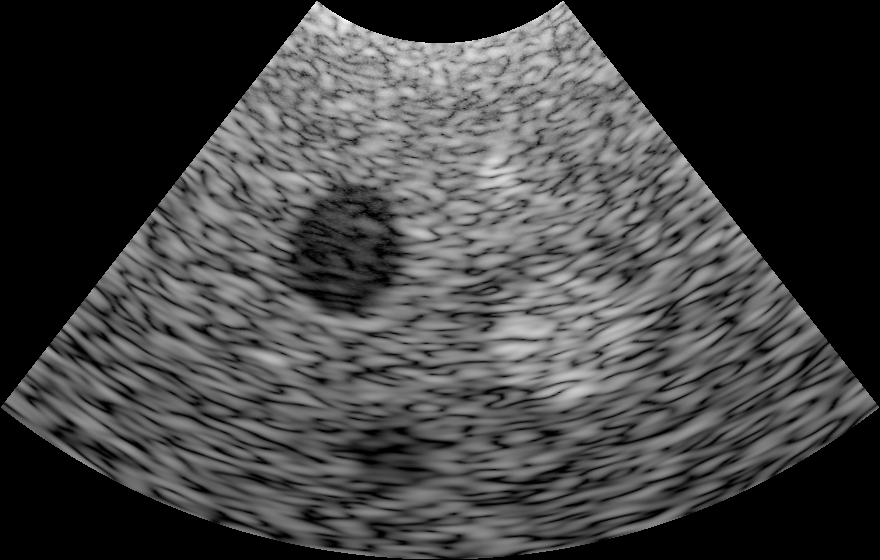
\includegraphics[width=\textwidth]{figures/us_raw.png}
  \caption{Simulated B-mode image with speckle}
  \label{fig:phantom-a}
\end{subfigure}
\hfill
\begin{subfigure}[b]{0.40\textwidth}
  \centering
  
\includegraphics[width=\textwidth]{figures/us_gt.png}
  \caption{Noise-free ground-truth reference}
  \label{fig:phantom-b}
\end{subfigure}
\caption{Output of the synthetic testbench. The ground-truth image (b) is
available only because the input originates from a simulator, and it enables the
reference-based metrics EPI and SSIM.}
\label{fig:phantom}
\end{figure}

The testbench operates on a $520\times220$ polar grid rendered to a
$560\times880$ display image over a $76^{\circ}$ sector, with a separable Gaussian
PSF ($\sigma_{\text{ax}}=2.6$, $\sigma_{\text{lat}}=3.4$ samples), attenuation
$\exp(-1.15\,r)$, a 40\,dB displayed dynamic range and bilinear scan conversion.



\subsection{Experimental Protocol}

A fixed protocol ensured fair comparison. A single testbench image is generated
with a fixed random seed so every filter sees identical input; Stage 1
normalisation is applied once and its output passed to all filters; each filter is
tuned by sweeping its principal control variable and selecting the setting with
highest CNR subject to $\mathrm{EPI}\geq0.90$ where achievable; the mask is
reapplied after filtering so the fan boundary is not contaminated by padding; and
all metrics are computed against identical ROIs and the same reference.

The final parameter values are recorded in Table~\ref{tab:params}.

\begin{table}[!htbp]
\centering
\caption{Final filter parameters used for the reported results.}
\label{tab:params}
\small
\begin{tabular}{L{3.4cm} L{9.0cm}}
\toprule
\textbf{Filter} & \textbf{Parameters}\\
\midrule
Median   & Window size $k = 9$\\
Lee      & Window size $k = 11$, $C_u = 0.523$\\
SRAD     & $400$ iterations, $\Delta t = 0.12$,
           $q_0(t) = 0.9/\sqrt{1+0.012\,t}$\\
NLM      & Patch $5\times5$, search radius $11$, $h = 0.16$\\
Wavelet  & Daubechies-4, 4 levels, soft threshold, $\sigma = 0.10$
           in log domain\\
CLAHE    & Clip limit $1.3$, tile grid $8\times8$\\
Unsharp  & $\lambda = 0.28$, $\sigma = 2.0$ pixels\\
\bottomrule
\end{tabular}
\end{table}

%=============================================================================
\chapter{RESULTS AND DISCUSSION}
\label{ch:results}
%=============================================================================

\section{Qualitative Results}

Figure~\ref{fig:comparison} shows all five filter outputs alongside the
unprocessed input, displayed with identical grey-level mapping.

The median filter reduces grain but rounds lesion boundaries and attenuates the
point targets, while the Lee filter preserves boundary definition noticeably
better at comparable suppression. NLM gives the smoothest tissue of any method,
though fine texture is lost. Wavelet thresholding retains texture but suppresses
the least speckle. SRAD, enlarged in Figure~\ref{fig:ba_srad}, strongly smooths
homogeneous tissue while keeping cyst and lesion boundaries sharp; the hypoechoic
nodule, barely visible in the input, becomes clearly discernible.

\begin{figure}[!htbp]
\centering

\includegraphics[width=0.56\textwidth]{figures/ba_srad.png}
\caption{SRAD, 400 iterations: input (left) and output (right). Homogeneous tissue
is strongly smoothed while the cyst and lesion boundaries remain sharp.}
\label{fig:ba_srad}
\end{figure}





\begin{figure}[!htbp]
\centering

\includegraphics[width=0.70\textwidth]{figures/comparison.png}
\caption{Side-by-side comparison of all five despeckling filters applied to the
same input image under identical display settings.}
\label{fig:comparison}
\end{figure}

\section{Quantitative Results}

Table~\ref{tab:results} reports the measured metrics, obtained on the testbench
image of Figure~\ref{fig:phantom-a} against the reference of
Figure~\ref{fig:phantom-b}.

\begin{table}[!htbp]
\centering
\caption{Measured image-quality metrics for all evaluated methods. Higher is
better in every column. The best value in each column is shown in bold.}
\label{tab:results}
\small
\begin{tabular}{L{3.3cm} C{1.7cm} C{2.0cm} C{1.7cm} C{1.7cm} C{1.9cm}}
\toprule
\textbf{Method} & \textbf{CNR} & \textbf{SNR}$_{\textbf{spk}}$ &
\textbf{EPI} & \textbf{SSIM} & \textbf{Speed}\\
\midrule
Original (raw)   & 1.78 & 4.28 & 1.000\textsuperscript{*} & 0.484 & ---\\
Median           & 2.45 & 7.07 & 0.759 & 0.625 & Very fast\\
Lee              & 2.58 & 7.55 & 0.943 & 0.667 & Fast\\
Wavelet          & 2.00 & 5.08 & 0.570 & 0.509 & Fast\\
NLM              & \textbf{3.03} & \textbf{9.77} & 0.806 & 0.728 & Slow\\
\textbf{SRAD}    & 2.98 & 9.29 & \textbf{0.955} & \textbf{0.744} & Moderate\\
\midrule
SRAD + CLAHE     & 2.27 & 5.02 & 0.827 & 0.640 & Moderate\\
\bottomrule
\multicolumn{6}{l}{\footnotesize\textsuperscript{*}Reference value by definition;
the raw image defines the unfiltered edge content.}
\end{tabular}
\end{table}

Figure~\ref{fig:bars} presents the same data graphically.\vspace{-4pt}

\begin{figure}[!htbp]
\centering

\includegraphics[width=0.66	extwidth]{figures/bar_results.png}
\caption{Measured contrast, speckle suppression and edge preservation for each
filter. The grey bar in each panel is the unprocessed reference.}
\label{fig:bars}
\end{figure}

\section{Discussion}

\subsection{Overall Performance}

Every filter improved both CNR and $\mathrm{SNR}_{\text{speckle}}$. The spread is
substantial: CNR gains range from $12\%$ (wavelet) to $71\%$ (NLM), and speckle SNR
gains from $19\%$ to $128\%$. The raw speckle SNR of $4.28$ exceeds the theoretical
$1.91$ of Equation~\eqref{eq:snr191} because the metric is computed after log
compression, which reduces the relative standard deviation; it remains valid as a
\emph{relative} indicator of smoothing.

\subsection{The Contrast--Edge Trade-Off}

The central finding is visible in the last two rows of the main block of
Table~\ref{tab:results}. NLM achieves the highest CNR ($3.03$) and speckle
suppression ($9.77$), but its EPI is only $0.806$. SRAD attains essentially the
same noise performance --- CNR $2.98$, a difference under $2\%$ --- while
retaining an EPI of $0.955$, some $18$ percentage points higher, and the highest
SSIM ($0.744$), indicating that its output is structurally closest to the true
anatomy. This is the quantitative expression of the trade-off identified in
Section~1.3.



Figure~\ref{fig:limits} demonstrates the failure mode. When smoothing strength is
increased well beyond the selected operating point, the hyperechoic lesion --- a
genuine finding --- is almost entirely erased. This is why the EPI criterion was
built into the parameter-selection loop of Figure~\ref{fig:flowchart}.





\subsection{Behaviour of Individual Filters}

The \textbf{median} filter shows the lowest EPI ($0.759$), consistent with theory:
as a fixed order statistic it applies the same operation regardless of local
content. The \textbf{Lee} filter performs markedly better on edges
($\mathrm{EPI}=0.943$) at similar noise suppression, validating the adaptive
weighting of Equation~\eqref{eq:leew}; its weakness is that the constant-$C_u$
assumption holds only for fully developed speckle. \textbf{SRAD} performs best
overall, as expected of the only method explicitly derived for multiplicative
speckle, its cost being the $400$ iterations that make it roughly an order of
magnitude slower than Lee. \textbf{NLM} gives the smoothest tissue, but its
patch-similarity weighting is content-agnostic near boundaries where few similar
patches exist, causing the observed edge softening; it was also the slowest method
evaluated. \textbf{Wavelet} thresholding preserved texture but removed the least
speckle: a more aggressive threshold raised the speckle SNR yet introduced ringing
near high-contrast boundaries, so the conservative setting was retained.

\begin{figure}[!htbp]
\centering

\includegraphics[width=0.66\textwidth]{figures/limits.png}
\caption{Consequence of over-smoothing. At excessive filter strength the
hyperechoic lesion (circled) is almost completely removed, despite the image
appearing subjectively cleaner.}
\label{fig:limits}
\end{figure}

\subsection{Effect of Contrast Enhancement}

The last row of Table~\ref{tab:results} records an important negative result.
Applying CLAHE and unsharp masking after SRAD \emph{reduced} CNR from $2.98$ to
$2.27$ and speckle SNR from $9.29$ to $5.02$, although the resulting image
appears subjectively crisper.



The explanation follows from Equations~\eqref{eq:cnr} and~\eqref{eq:snr}: both
operators amplify local variance, and since $\sigma_\ell$ and $\sigma_b$ appear in
the denominators, any such increase depresses the scores even when the mean
separation $|\mu_\ell-\mu_b|$ is unchanged. Stage 3 must therefore be treated as a
\emph{display-only} operation, with Stage 4 metrics computed on the Stage 2 output
and enhancement applied afterwards purely for presentation.

\subsection{Summary of Findings}

\begin{enumerate}[leftmargin=*,itemsep=0pt,topsep=2pt]
\item All five classical filters suppress speckle measurably; no machine learning
      is required for substantial improvement.
\item SRAD offers the best balance, nearly doubling CNR ($1.78 \to 2.98$) and more
      than doubling speckle SNR ($4.28 \to 9.29$) while retaining $95.5\%$ of edge
      information and achieving the highest SSIM.
\item NLM marginally exceeds SRAD in noise suppression, but at significant cost in
      edge fidelity and computation time.
\item Contrast enhancement improves subjective appearance yet degrades objective
      metrics, so it is excluded from the measurement path.
\item \textbf{SRAD with the parameters of Table~\ref{tab:params} is the
      recommended default filter.}
\end{enumerate}



%=============================================================================
\chapter{CONCLUSION AND FUTURE WORK}
\label{ch:conclusion}
%=============================================================================

\section{Conclusion}

This report has presented the design, implementation and evaluation of the Post
Image Processing module of NITK-UsoundSim, which converts the raw log-compressed,
scan-converted B-mode image into a display-ready image with suppressed speckle.

Speckle was shown to be a deterministic consequence of coherent imaging rather
than additive electronic noise, and therefore not removable by improved hardware.
The Rayleigh envelope statistics of fully developed speckle were used both to
derive the Lee constant $C_u = 0.523$ and to define the speckle SNR metric.

A four-stage pipeline was designed --- depth gain normalisation, despeckle
filtering, contrast restoration and quality assessment --- with a documented
interface allowing independent development. Five classical filters were
implemented in Python and compared under an identical protocol on a synthetic
testbench supplying a ground-truth reference.

The measured results identify SRAD as the preferred operator. It raised the
contrast-to-noise ratio from $1.78$ to $2.98$ and the speckle signal-to-noise
ratio from $4.28$ to $9.29$, while retaining an edge-preservation index of
$0.955$ and achieving the highest structural similarity of any method tested
($0.744$). Non-Local Means achieved marginally better noise suppression but lost
substantially more edge information and was considerably slower.

A secondary finding is that contrast enhancement, while improving subjective
appearance, systematically depresses variance-normalised metrics, and must
therefore sit outside the measurement path.

\section{Limitations}

Three limitations qualify these conclusions.

First, all results were obtained on a synthetic testbench rather than on
production output. The testbench reproduces the properties agreed in the interface
contract, but the parameters of Table~\ref{tab:params} will require re-tuning
against production data.

Second, the parameters were tuned on a single phantom. Generalisation across
imaging depths, sector angles and tissue types has not been established.

Third, computational cost was assessed only qualitatively. SRAD at $400$
iterations and NLM are both too slow for real-time operation, restricting the
present implementation to offline processing.

\section{Future Work}

\textbf{Validation against production data.} Repeat the evaluation on images from
the upstream module and re-tune the parameters accordingly.

\textbf{Adaptive parameter selection.} Select filter strength automatically from
an estimate of the local speckle scale, allowing the module to adapt to varying
imaging conditions rather than using one fixed configuration.

\textbf{Computational acceleration.} The SRAD update of
Equation~\eqref{eq:sradupdate} is a local stencil operation and is well suited to
GPU execution; a parallel implementation would make real-time operation feasible.

\textbf{Extension of the metric set.} The generalised contrast-to-noise ratio
\cite{rodriguez2020gcnr} is insensitive to monotonic intensity transformations and
would not exhibit the enhancement artefact of Section~5.3.5. Resolution metrics
based on the full width at half maximum of the point targets would further
strengthen the evaluation.

\textbf{Learning-based despeckling.} Convolutional and adversarial networks report
performance beyond classical filters, but supervised training requires paired
noisy and clean images that clinical ultrasound cannot provide. As Abadi
\emph{et al.} \cite{abadi2020vct} observe, a validated simulator supplies exactly
such paired data at scale; the testbench developed here already generates the
required references.

%=============================================================================
{\small\setstretch{1.08}
\bibliographystyle{ieeetr}
\bibliography{references}}
\addcontentsline{toc}{chapter}{References}

\end{document}
